% NQS architecture for the fermionic 3D toric code: the 2026-08-07..10 discoveries,
% explained conceptually. Companion/sequel to notes/fermionic_sign_problem.tex
% (background: 2D warm-up, sign-problem definitions, origin of the fTC signs,
% the positive-sector trap). This document starts where that one ends.
% Compile: pdflatex fermionic_architecture.tex  (twice, for refs)
\documentclass[11pt]{article}
\usepackage[margin=1.1in]{geometry}
\usepackage{amsmath,amssymb,amsthm}
\usepackage{booktabs}
\usepackage{array}
\usepackage{tikz}
\usetikzlibrary{positioning,arrows.meta,calc}
\usepackage[colorlinks=true,linkcolor=blue!60!black,citecolor=blue!60!black,urlcolor=blue!60!black]{hyperref}
\usepackage{microtype}
\usepackage{graphicx}
\setlength{\emergencystretch}{2.5em}  % rescue lines with unbreakable \texttt paths

\newcommand{\Av}{A_v}
\newcommand{\Bp}{B_p}
\newcommand{\Bt}{\tilde B_p}
\newcommand{\ket}[1]{|#1\rangle}
\newcommand{\bra}[1]{\langle#1|}
\newcommand{\braket}[2]{\langle#1|#2\rangle}
\newcommand{\sx}{\sigma^x}
\newcommand{\sy}{\sigma^y}
\newcommand{\sz}{\sigma^z}
\newcommand{\GF}{\mathrm{GF}(2)}
\newcommand{\file}[1]{\texttt{#1}}
\newcommand{\circled}[1]{\textcircled{\raisebox{-0.5pt}{\scriptsize #1}}}

\title{The fermionic NQS architecture:\\
from the sign trap to exact ground states at any $L$\\
{\large a conceptual companion for the finite-field design discussion}}
\author{toric-code-nqs project notes}
\date{August 10, 2026}

\begin{document}
\maketitle

\begin{abstract}
\noindent
The background note \cite{SignNote} ends at a cliffhanger: the fermionic 3D
toric code (fTC) is sign-full at zero field, cold-start VMC provably traps at
the positive-sector optimum ($L=2$: $E=-22.52$ vs.\ $-32$), and a list of
candidate strategies is on the table. This document explains what happened
next (2026-08-07\,..\,10): which strategies were tried, precisely how each
failed, and the design that emerged --- signs written \emph{analytically} into a
token-quadratic phase head by $\GF$ linear algebra ($L=2$ exact,
$\delta=1.3\times10^{-7}$); a second, previously invisible discrete channel
(flux superselection sectors) discovered at $L=3$ and cured by an equally
analytic, zero-parameter flux penalty ($L=3$ exact, $\delta=3.8\times10^{-8}$);
a no-go theorem explaining why no universal local convolutional sign head can
exist; and an any-$L$ closed-form construction of the head (signs certified
exact at $L=2..6$) that makes the design production-ready. The recurring
lesson --- the \emph{doctrine} --- is stated up front, and the final section turns
it into concrete design choices for the perturbed model, where NQS is the only
available method.
\end{abstract}

\tableofcontents

%=====================================================================
\section{Orientation: what this document is, and the doctrine}
\label{sec:orientation}

This is a pedagogical companion, not a paper draft. It assumes the background
note \cite{SignNote}: the model definition ($\Bt = Z(\partial p)\,
\sx_{e_+}\sx_{e_-}$ with the $\sx$ pair on body-diagonal corner edges, stars
untouched, PBC; see also \file{notes/handoff\_fermionic\_tc.md}), why the fTC
is sign-full already at $h=0$, the QMC-vs-VMC taxonomy of sign problems, and
the diagnosis of the positive-sector trap
(\file{notes/fermionic\_plateau\_diagnosis.md}). None of that is repeated
here. What \emph{is} covered: the architecture discoveries of
2026-08-07\,..\,10, made in a fast and (from the outside) confusing sequence of
runs, bugs, and reversals --- reconstructed here as the conceptual map it turned
out to be. Primary sources: the three BLOG entries of 2026-08-07 (morning:
sign trap; later: phase head; night: $L=3$ and ghost sectors), the plan note
\file{notes/fermionic\_next\_steps.md}, the obstruction note
\file{notes/fermionic\_stencil\_obstruction.md}, and commits
\texttt{876ccca}\,..\,\texttt{8986de0}.

\paragraph{The doctrine.}
Every result in this document is an instance of one principle, discovered
once for signs and then rediscovered, independently and painfully, for flux
sectors:

\begin{center}
\fbox{\parbox{0.9\textwidth}{\centering\itshape
Every discrete/topological channel of the wavefunction must be solved
algebraically ($\GF$) and written into the ansatz as data.\\
Optimizers touch only the smooth amplitude channel.}}
\end{center}

\noindent
The intuition: gradient-based optimizers (SR included) are interpolators of
smooth landscapes. A stabilizer sign structure or a superselection-sector
label is not a smooth landscape --- it is a finite, exactly computable,
combinatorial object. Asking SR to \emph{find} it produces the failure modes
of Sec.~\ref{sec:options}; asking SR to merely \emph{preserve} it while it
does honest amplitude work produces machine-precision ground states.

\paragraph{Headline results (all $h=0$, PBC, exact $E_0=-4L^3$).}
$L=2$: $E=-32.0000$, $\delta=1.3\times10^{-7}$, Vscore $2\times10^{-8}$ (run
\texttt{\dots\_ph\_polishANA}). $L=3$: $E=-107.99999592(6)$,
$\delta=3.8\times10^{-8}$, Vscore $2\times10^{-7}$, $\langle\Bt\rangle =
1.000000025$ (run \texttt{\dots\_ph\_fp6\_polishANA}, $\sim$20\,s/step).
Sign structure certified exact at $L=2..6$ by $10^4/10^4$ fresh-class
certificates. Amplitude runs at $L=4/5/6$ against anchors $-256/-500/-864$
are in flight; results \textbf{[PENDING]} (Sec.~\ref{sec:status}).

\paragraph{Timeline.}
Table~\ref{tab:timeline} is the debugging blizzard in compressed form; the
rest of the document unpacks each row.

\begin{table}[h]
\centering\small
\begin{tabular}{@{}p{0.13\textwidth}p{0.47\textwidth}p{0.32\textwidth}@{}}
\toprule
2026- & what happened & what it taught \\
\midrule
08-06 & cold-start benchmark: both production configs converge to
$E=-22.52$ vs.\ $-32$ & ansatz expressive enough; \emph{SR} is the failing
component \\
08-07 a.m. & trap diagnosed: positive-sector optimum, escape-proof
\cite{SignNote} & sign problem migrates into the optimizer \\
08-07 & supervised pre-fit ladder: joint fits, head-only fits, zero-init,
bare-head SGD --- four distinct failure modes (Sec.~\ref{sec:options}) &
optimizers smear, pollute, stall, or locally minimize the sign channel \\
08-07 & \textbf{analytic $\GF$ head}: $\theta$ computed, not trained
$\to$ $L=2$ exact, $\delta=1.3\times10^{-7}$ & doctrine, first confirmation \\
08-07 night & sampled-class solve at $L=3$; polish plateaus at $-89.97$ with
\emph{perfect} signs; MCMC census: 99.8\% weight in ghost flux sectors;
\textbf{flux-penalty head} $\to$ $L=3$ exact, $\delta=3.8\times10^{-8}$ &
doctrine, second confirmation: flux sectors are a discrete channel too \\
08-07 & stencil study: no universal local TI sign form; TI representative
exists iff $L$ odd & the dense per-size head is physics, not a shortcut \\
08-09 & C-form pullback: analytic $\theta$ at \emph{any} $L$, no solving;
frozen head (\texttt{constants}); certificates $L=2..6$ & the ``per-size
dense'' cost objection evaporates \\
08-10 & penalty as one matmul (was 78\,min/step at $L=6$);
\texttt{--chains\_up}; $L=4/5/6$ launched & production hardening
(Sec.~\ref{sec:lessons}) \\
\bottomrule
\end{tabular}
\caption{The 2026-08-07..10 sequence. Commits \texttt{876ccca}..\texttt{8986de0}.}
\label{tab:timeline}
\end{table}

%=====================================================================
\section{The starting point: a sign that is exactly knowable}
\label{sec:start}

Two facts from \cite{SignNote} carry the whole story; everything else in this
section is a reminder.

\paragraph{Fact 1: the $h=0$ ground state is a \emph{signed stabilizer
state}, and its sign is a $\GF$ quadratic form over flux tokens.}
Define the flux tokens
\begin{equation}
t_p(s) \;=\; \prod_{e\in\partial p} s_e \;=\; \varepsilon_p(s)\in\{\pm1\},
\qquad p = 1,\dots,N_p=3L^3 ,
\label{eq:tokens}
\end{equation}
the plaquette-boundary $z$-parities of a configuration $s$. Propagating the
stabilizer eigenvalue equations from $\ket{0\cdots0}$ enumerates the
ground-state support with exact signs (at $L=2$: $2^{15}$ states, 56\%/44\%
positive/negative). Structurally, sign-changing moves (decoration-pair flips
with odd boundary overlap) always change tokens, and token-preserving moves
(stars) never change signs --- so the sign is an exact \emph{function of the
token vector}, and by the general theory of stabilizer states that function
is a $\GF$ quadratic form: on the support,
\begin{equation}
\mathrm{sign}\,\psi(s) \;=\; (-1)^{\,q(t(s))},
\qquad q(t) = \ell\cdot t + t^{\!\top} Q\, t \ \ \text{over } \GF .
\label{eq:quadform}
\end{equation}
At $L=2$ the support collapses to $64 = 2^6$ token classes, each carrying one
sign. The number $6$ will matter: it is $\dim V$, the dimension of the
physical token space (Sec.~\ref{sec:ghost}).

\paragraph{Fact 2: cold-start VMC converges --- to the wrong thing, robustly.}
Both production hyperparameter sets converge at $L=2$ to $E=-22.52$
($\delta=29.6\%$), the optimal wavefunction confined to the positive-sign half
of the support, with SR polishing this impostor to Vscore $10^{-9}$; a
guard-off escape probe (400 hot iterations) attempted crossings and relaxed
back. Every smooth path to the true state first raises energy and variance;
the sampler never visits the negative half; the trap is escape-proof in
practice. The sign problem has not disappeared --- it has migrated from the
sampler into the optimizer.

\paragraph{The question as of 08-07 morning.}
Fact 1 says the discrete data is \emph{cheap to know}; Fact 2 says the
optimizer will not find it. The engineering question was therefore never
``can the network represent the signs'' (it can; supervised fits reach 100\%
on trained states in $\sim$100 Adam steps) but: \emph{through which channel,
set by what procedure, does the exact sign structure enter the ansatz so that
subsequent SR training helps rather than harms?} Several plausible answers
were on the table. All but one failed, each for a different and instructive
reason.

%=====================================================================
\section{The options and their fates}
\label{sec:options}

The experimental setup, common to all rungs of the ladder ($L=2$, $h=0$):
supervised targets from the exact sign map; the \emph{extrapolation probe} is
a class-level hold-out --- train on 48 of the 64 token classes, test on the 16
unseen classes. Getting held-out classes right is the only thing that
matters: it distinguishes ``memorized the training signs'' from ``represents
the quadratic form,'' and only the latter survives contact with VMC (which
immediately drives the state through configurations no pre-fit ever saw).

The candidate architectural channel, implemented on 08-07
(\texttt{--phase\_head}, commit \texttt{4a43811}): a \emph{token-quadratic
phase head}, a parallel branch summed into $\log\psi$,
\begin{equation}
\Delta\log\psi(s) \;=\; i\,\varphi(t),\qquad
\varphi(t) \;=\; \sum_p \theta_p\, t_p \;+\; \sum_{p,q} \theta_{pq}\, t_p t_q ,
\label{eq:head}
\end{equation}
computed from the \emph{raw-input} tokens \eqref{eq:tokens}, not from learned
features. By \eqref{eq:quadform} this hypothesis class contains the exact
$h=0$ sign structure (with $\theta$ the $\pm1$-variable transcription of
$(\ell,Q)$); at $L=2$ it has $24+576=600$ parameters. The head's existence,
however, settles nothing --- the ladder below is entirely about \emph{how
$\theta$ gets its values}. See
\file{analysis/fermionic\_h0\_prefit\_ladder.ipynb} for the curves;
\file{analysis/prefit\_phase\_head.py} is the tool.

\subsection{(a) Joint supervised pre-fit of trunk (+ head): credit smearing}
Fit the network's total phase output to the exact signs, all parameters
trainable. Result: 100\% on trained states, but 14/16 held-out classes
without the head and --- pointedly --- \emph{13}/16 with it. Gradient descent
distributes (``smears'') the sign-fitting credit across trunk and head; the
head is present but never forced to own the structure, so the network learns
an approximation of the rule rather than the rule, even though 48 classes
over-determine the 600-parameter form. The SR polish from these warm starts
then exposed two deeper pathologies:
\begin{itemize}
\item \textbf{SR pays for sign defects; it never repairs them.} The 62/64-
and 64/64-sign warm starts blew straight through the old $-22.52$ trap and
froze at $E=-31.30$ and $-31.64$ respectively ($\delta = 2.2\%$, $1.1\%$):
each residual sign error is a fixed energy tax the amplitude optimizer
routes around but cannot remove.
\item \textbf{Even perfect signs drift.} A pre-fit shapes signs on the
support only (its raw energy is $\approx-10.9$); early SR does violent
amplitude work draining off-support weight, and the smeared trunk-resident
sign representation loses fidelity under exactly that deformation. Perfect
signs stored the wrong way are perishable.
\end{itemize}

\subsection{(b) Head-only fit over a random complex trunk: phase pollution}
Freeze the trunk, fit only $\theta$. Result: 11/16 --- \emph{worse}. The
randomly initialized complex trunk carries $O(0.3\,\mathrm{rad})$ phases that
are not quadratic in the tokens; the head, fitting total phase, absorbs their
projection onto its basis and then confidently extrapolates that bias to
unseen classes. The head can only be exact over a trunk that contributes
\emph{zero} phase.

\subsection{(c) Real trunk + zero-initialized head: an exact saddle}
So make the trunk exactly real and let the head learn from zero. Result:
frozen at baseline accuracy, gradient identically zero. Every sensible sign
loss is an even function of the phases (flipping all phases' signs cannot
change a cost built from $\cos$ of phase differences), so $b\equiv0$ is a
stationary point of \emph{any} such loss. The honest starting point for the
sign channel is, by symmetry, a point where gradient descent receives no
instruction.

\subsection{(d) Noise-seeded SGD on the bare 600-parameter head: local minima}
Break the saddle with noise and descend the cosine loss of the head alone.
Result: plateaus at 62/64 classes. A linear-in-parameters phase model under a
cosine loss is a phase-retrieval problem, and phase retrieval landscapes have
genuine non-global minima; the earlier big-network fits only ever escaped
these by overparameterization --- which is exactly the smearing of (a). Two
wrong classes out of 64 sounds close; as a sign structure it is a permanent
$O(1)$ energy tax (cf.\ the polish freezes above).

\subsection{(e) What worked: $\theta$ computed, not trained}
Each sampled support configuration with its exact sign contributes one linear
equation over $\GF$ for the unknowns $(\ell,Q)$ of \eqref{eq:quadform}. Solve
the system from 48 class labels by Gaussian elimination; transcribe
$(\ell,Q)$ into $\theta$; \emph{write} $\theta$ into the head. Result: 16/16
held-out classes, 100\% on all $32{,}768$ support states, zero training
steps. The SR polish from this initialization passed $-31.96$ by step 20 and
converged to $E=-32.0000$, $\delta=1.3\times10^{-7}$, Vscore $2\times10^{-8}$
--- through the trap region without a wobble (run
\texttt{\dots\_ph\_polishANA}, commit \texttt{195491e}).

Two control experiments complete the picture. First, a cold start \emph{with}
the head present but zero-initialized still traps at $-22.52$: the head fixes
representability and storage, not the descent path --- an unused hypothesis
class is furniture. Second, the analytic $\theta$ is robust precisely where
(a) was fragile: SR's amplitude work never touches an explicitly stored
$\theta$, so the early off-support drain cannot degrade it.

\begin{table}[h]
\centering\small
\setlength{\tabcolsep}{4.5pt}
\begin{tabular}{@{}llll@{}}
\toprule
option & held-out & SR polish & failure mode \\
\midrule
(a) joint trunk-only fit & 14/16 & $-31.64$ ($\delta=1.1\%$) & credit smearing; drift \\
(a$'$) joint trunk+head fit & 13/16 & $-30.15$ ($\delta=5.8\%$) & smearing, worse \\
(b) head over random trunk & 11/16 & --- & trunk phase pollution \\
(c) real trunk, $\theta=0$ & frozen & --- & exact saddle ($b\equiv0$) \\
(d) SGD on bare head & 62/64 cls. & --- & phase-retrieval local minima \\
(e) \textbf{analytic $\GF$ solve} & \textbf{16/16} & $\mathbf{-32.0000}$
($\delta=1.3\times10^{-7}$) & --- \\
\midrule
control: cold start, $\theta=0$ & --- & $-22.52$ ($\delta=29.6\%$) &
the trap, unchanged \\
\bottomrule
\end{tabular}
\caption{The $L=2$ ladder (BLOG 2026-08-07, ``later'' entry). Each failure
isolates one requirement; jointly they force option (e).}
\label{tab:ladder}
\end{table}

\paragraph{Why this is physics, not a trick.}
The head with analytic $\theta$ \emph{is} the lattice-bosonization phase
factor of Chen--Kapustin \cite{ChenKapustinRadicevic2018,ChenKapustin2019}: a
discrete gauge structure $e^{i\pi q(\mathrm{flux})}$ attached to flux
configurations to encode fermionic statistics. It is the wavefunction-side
counterpart of the operator-side Clifford disentangler discussed in
\cite{SignNote} --- but cheaper, since the Hamiltonian, sampler, and field
terms stay untouched. It is also the best-case instance of the explicit
phase-ansatz philosophy of Szab\'o--Castelnovo \cite{SzaboCastelnovo2020}:
here the explicit phase is not a physically motivated guess but the exact
answer.

%=====================================================================
\section{Scaling to $L=3$: the second discrete channel}
\label{sec:L3}

$L=2$ leaned on a luxury that dies immediately: full enumeration of the
$2^{15}$-state support. Scaling the recipe required replacing enumeration ---
and then, unexpectedly, revealed that the sign channel was not the only
discrete channel in the problem.

\subsection{The sampled-class generator}
\label{sec:sampled}

The replacement (commit \texttt{ff3d1c0}, \file{analysis/prefit\_phase\_head.py})
generates supervised sign equations without ever enumerating anything: draw a
uniform random subset $x$ of the $3L^3$ decorated plaquette operators, apply
them to $\ket{0\cdots0}$ accumulating the exact sign via the propagation
rules ($\psi(s\oplus d_p)=\varepsilon_p(s)\psi(s)$; commutation makes the
order irrelevant, and stars are provably irrelevant --- they change neither
tokens nor signs). Each draw yields one $\GF$ equation for $(\ell,Q)$; an
online augmented elimination absorbs rows, detects contradictions, and stops
when the rank saturates.

The rank tells you it is working: the token vectors reachable from
$\ket{0\cdots0}$ span a space $V$ of dimension $d$, and a quadratic form on a
$d$-dimensional $\GF$ space has exactly $d(d+1)/2$ independent coefficients.
Observed: rank saturates at $21 = 6\cdot7/2$ at $L=2$ ($d=6$; $2^6=64$
classes, matching enumeration) and at $666 = 36\cdot37/2$ at $L=3$ ($d=36$),
after 1168 draws, zero contradictions. The certificate is the point:
$10^4/10^4$ correct signs on fresh samples, \emph{every one of them a
never-before-seen token class} (about $2^{36}\approx7\times10^{10}$ classes
exist at $L=3$). Any consistent solution of a rank-saturated system agrees on
the whole span --- the certificate verifies exactness, not generalization.

\subsection{The ghost-sector trap}
\label{sec:ghost}

With exact $L=3$ signs in the head, the polish was expected to close. It
plateaued at $E=-89.97$ (exact: $-108$) --- while every sign-channel diagnostic
came back \emph{perfect}: 100\% sign accuracy on fresh support samples,
uniform support amplitudes, 0.4\% head drift. The state was flawless and the
energy was 17\% wrong.

The resolution came from an MCMC census against the exact solution:
\textbf{99.8\% of the sampled weight sat in wrong flux sectors}, at full
on-orbit amplitude. The mechanism needs one structural observation. A
decoration-pair flip $d_p$ changes the token vector by a fixed pattern --- the
$p$-th column of the $\GF$ \emph{token-flip map} $M$,
$M_{qp}=|\partial q\cap d_p| \bmod 2$. The token vectors reachable from the
all-up state are therefore exactly the column space $V=\mathrm{col}\,M$ (of
dimension $d$, the same $d$ as above), and the full token space
$\{0,1\}^{N_p}$ shatters into $2^{N_p-d}$ cosets of $V$ --- $2^{45}$ of them at
$L=3$. These cosets are superselection sectors of the $h=0$ dynamics:
\emph{every} move in the sampler's repertoire (star flips, pair-cluster
flips) conserves the coset. Now the conspiracy:
\begin{itemize}
\item \textbf{Sampling:} each chain starts at a random configuration, i.e.\
in a random coset --- and can never leave it.
\item \textbf{Representation:} the trunk's Wilson-token architecture has no
cheap feature distinguishing the physical coset from a ghost coset, so the
warm-started network assigns ghost configurations healthy on-orbit
amplitudes; ghosts outnumber the physical sector $2^{45}$:$1$.
\item \textbf{Optimization:} SR, fed samples from ghost cosets, faithfully
converges to the optimal state \emph{of the sector it can see}
($\langle\Bt\rangle=0.777$ is near-optimal there:
$E=-27-81\times0.777\approx-89.9$).
\end{itemize}
And the reason nobody noticed for a day: every standard diagnostic is
structurally blind to it. $\langle\Av\rangle=1$ is \emph{architecturally
vacuous} --- star flips do not change tokens, so any token-functional ansatz
satisfies the star symmetry identically, in every sector.
$\mathrm{Im}\langle E\rangle=0$ because the analytic head generalizes
\emph{consistently} into ghost sectors (it is a form on all of token space).
And the Vscore was small because the state genuinely was a near-eigenstate ---
of the restriction of $H$ to the wrong sector. This is the positive-sector
trap of \cite{SignNote} one level up: not signs this time, but sector labels;
another discrete, exactly-knowable structure the optimizer was implicitly
asked to discover, and didn't.

\subsection{The flux-penalty head: an analytic, zero-parameter cure}
\label{sec:fluxpenalty}

The doctrine, applied again. Which sector a configuration is in is $\GF$
data: the physical sector $V=\mathrm{col}\,M$ is cut out by the null space of
$M^{\!\top}$ --- a basis of token subsets $c$ whose parities
\begin{equation}
u_c(s) \;=\; \prod_{p\in c} t_p(s) \;\in\;\{\pm1\}
\label{eq:gausslaw}
\end{equation}
are conserved by every pair move and equal $+1$ exactly on the physical
sector. Physically these are the lattice Gauss laws --- closed-surface flux
parities; ghost cosets violate at least one. Computed once from the geometry
(\file{tc3d/fermionic\_decoration.py}, \texttt{flux\_constraint\_masks}),
their counts are $N_p-\dim V$:
\begin{center}
\begin{tabular}{@{}lccccc@{}}
\toprule
$L$ & 2 & 3 & 4 & 5 & 6\\
\midrule
$N_p=3L^3$ & 24 & 81 & 192 & 375 & 648\\
$\dim V$ & 6 & 36 & 94 & 200 & 358\\
Gauss masks & 18 & 45 & 98 & 175 & 290\\
\bottomrule
\end{tabular}
\end{center}
The head (\texttt{--flux\_penalty}~$\kappa$, commit \texttt{43415f4}) then
subtracts a \emph{fixed} $\kappa$ from $\mathrm{Re}\log\psi$ per violated
parity:
\begin{equation}
\Delta \mathrm{Re}\log\psi(s) \;=\; -\kappa\,\#\{c : u_c(s)=-1\}
\;=\;\frac{\kappa}{2}\Big(\sum_c u_c(s) - N_c\Big),
\label{eq:penalty}
\end{equation}
suppressing each violation's probability by $e^{-2\kappa}\approx
6\times10^{-6}$ at the working value $\kappa=6$. Zero parameters, never
trained --- an analytic sector projection that leaves checkpoints
tree-compatible with the penalty on or off.

The validation was deliberately \emph{training-free}: attach the penalty to
the plateaued checkpoint and just measure. On-sector weight jumped from 0.2\%
to 100.0\% and $\langle H\rangle=-107.916(31)$ with no retraining ---
three-digit agreement from a diagnostic flag flip. A 150-step SR polish then
closed it, in about 40 steps, to
\[
E=-107.99999592(6),\qquad \delta=3.8\times10^{-8},\qquad
\text{Vscore } 2.0\times10^{-7}
\]
(run \texttt{\dots\_ph\_fp6\_polishANA}; results in
\file{results/fermionic\_h0/}). The doctrine had now been confirmed twice, on
two different discrete channels, with the same signature each time: the
optimizer converges beautifully inside whatever subspace it is handed; the
discrete data deciding \emph{which} subspace must be computed and installed,
never learned.

%=====================================================================
\section{Why no universal local convolutional sign head exists}
\label{sec:stencil}

Before scaling further, plan item \circled{2} asked the natural economy question: the
analytic head is dense ($N_p+N_p^2$ coefficients per size); does a \emph{local,
translation-invariant stencil} representative exist --- solve $O(1)$ couplings
once at small $L$, convolve at any $L$? The answer is a clean \textbf{no},
and the way it fails is physics. (Sources:
\file{notes/fermionic\_stencil\_obstruction.md} and
\file{analysis/stencil\_phase\_head.py}, commit \texttt{8b4ec59}.)

\paragraph{Where the sign \emph{is} local and TI: application variables.}
Let $x\in\GF^{N_p}$ record which decorated plaquettes were applied to
$\ket{0\cdots0}$. Commutativity makes the accumulated sign a well-defined
quadratic form, and it is \emph{analytic}:
\begin{equation}
\mathrm{sign}(x) = (-1)^{\sum_{p<q} C_{pq}x_p x_q},
\qquad C_{pq} = |\partial p \cap d_q| \bmod 2 ,
\label{eq:Cform}
\end{equation}
with $C$ symmetric (commutation makes odd overlap reciprocal), range exactly
one lattice unit, translation invariant --- each plaquette couples to exactly
8 neighbors --- and requiring no solving at all. Verified by sampling,
3000/3000 at $L=2,3,4$. This is the operational, bosonization-phase form of
the sign.\footnote{A pleasing coincidence of the geometry: the same $\GF$
matrix plays both roles in this story --- $C$ of \eqref{eq:Cform} \emph{is} the
token-flip map $M$ of Sec.~\ref{sec:ghost} ($M_{qp}=|\partial q\cap
d_p|=C_{qp}$). The matrix that generates the signs also delimits the physical
sector.}

\paragraph{Where it is not: state variables.}
The network, however, sees the state, not the application history: $x$ is
exposed only through linear screens --- the tokens $t=Mx$, or the bits $s$
($x$ up to $\ker M$ and the star span). Writing \eqref{eq:Cform} as a form in
state variables means pulling $C$ back through a (pseudo)inverse of a local
map, and inverses of local maps are generically nonlocal (think $\nabla^{-2}$).
The empirical campaign (sampled class equations, joint $\GF$ feasibility,
fresh-sample certificates) made this precise:
\begin{itemize}
\item tokens, range 1, solved at $L=3$ alone: feasible, 5000/5000 --- but a
\emph{folded gauge accident}: the same stencil deployed verbatim at $L=4,5$
scores $\sim$50\% = coin flip;
\item joint solve over $L=3{+}4$ (tokens or bits), range 1: infeasible
($\sim$2000 inconsistent rows);
\item bits, $L=4$ alone: infeasible at range 1, 1.5, 2 (= the whole torus) ---
\textbf{no TI form exists at $L=4$ at all}, and period-2 sublattice
(cell-parity) enrichment does not rescue it (1210 bad rows);
\item bits, $L=5$: infeasible at range 1, \emph{feasible} at full range
(residual 0, 1000/1000) with couplings reaching $|\Delta|\approx L/2$ --- TI
but nonlocal.
\end{itemize}

\paragraph{The parity theorem: why odd $L$ is special.}
The state is TI, so if $q$ is a valid sign form, so is every translate
$q\circ T_g$, and differences of valid forms vanish on the class space $V$.
Summing over the translation group, $\sum_g q\circ T_g = |G|\cdot q +
(\text{form vanishing on }V)$ over $\GF$. For $|G|=L^3$ \emph{odd}, the sum
is itself a manifestly TI valid representative --- existence guaranteed, and
$L=3,5$ confirm. For even $L$ the argument collapses ($|G|\cdot q = 0$), and
empirically no TI representative exists at $L=4$. Locality, meanwhile, fails
across sizes even when TI holds.

\paragraph{Reading: a Kasteleyn/spin-structure obstruction.}
This is exactly the classical pattern for encoding fermion signs in local
lattice data: a Kasteleyn orientation exists locally everywhere, but on an
even torus no translation-invariant one exists --- one must insert a
codimension-1 defect seam (the antiperiodic spin structure). Our form
reproduces it: locally trivial to write down \eqref{eq:Cform}, globally, as a
function of the state, demanding odd size or TI-breaking seam data. The
hardness of the fTC sign structure is a \emph{global topological} feature.
Consequence for architecture: the per-size dense analytic head is not an
unfortunate stopgap but the correct design --- and Sec.~\ref{sec:anyL} shows
it is also cheap. (A seam-decorated stencil at even $L$ remains an
interesting compression follow-up, not a blocker.)

%=====================================================================
\section{The any-$L$ construction and the production stack}
\label{sec:anyL}

\subsection{The C-form pullback: exact $\theta$ at any $L$, no solving}
\label{sec:pullback}

The sampled-class solve of Sec.~\ref{sec:sampled} is poly($L$) but still a
solve. The obstruction analysis handed over something better: the sign is
\emph{already known analytically} in application variables, Eq.~\eqref{eq:Cform}.
All that is missing is transport to token space --- find $q(t)$ with
$q(Mx)=\tilde q(x)$ on the physical sector. That needs a right-inverse of
$M$ over $\GF$: run Gaussian elimination on $M$'s columns with \emph{full-RREF
preimage tracking}, so that any $t\in V$ decomposes as the XOR of tracked
preimages over its pivot coordinates, $x(t)$ linear in $t$; substituting into
$\tilde q$ gives $q(t)=\ell\cdot t + t^{\!\top}Qt$ supported on pivot
coordinates only. Values off $V$ are irrelevant --- the flux penalty has
already exiled those sectors. (Commit \texttt{7e9c59e},
\texttt{--analytic\_C} in \file{analysis/prefit\_phase\_head.py}; stored
forms in \file{results/fermionic\_h0/solved\_form\_L*.json}.)

One instructive bug deserves its paragraph, as a lesson about exact-algebra
code. The first implementation reduced each new column only while its lowest
set bit was an existing pivot --- leaving rows that were eliminated but not
\emph{fully} reduced, i.e.\ not in RREF. Preimage extraction assumes pivot
coordinates are cleanly separated; non-RREF rows silently corrupt it. At
$L=2$ the pivot structure happened to mask the bug; at $L\ge3$ the
certificates came back at exactly 50\% --- chance --- with no error anywhere.
Exact discrete pipelines fail loudly only if you build the loud part
yourself: the fresh-class certificate, not the solver, is what caught this.

With the fix: certificates $10^4/10^4$ fresh classes at every $L=2..6$, CNN
sign accuracy $1.000000$ each, and at $L=2$ additionally exact on the full
$32{,}768$-state enumeration. Exact signs at any size, in closed form, in
seconds.

\subsection{The frozen head: signs as constants, invisible to the optimizer}
\label{sec:frozen}

If $\theta$ is analytic and must never be trained, it should not be a
parameter at all. The flag \texttt{--phase\_head\_frozen} stores $\theta$ in a
flax \texttt{constants} collection (part of \texttt{model\_state}): carried by
checkpoints and \texttt{--init\_from} like any weight, but invisible to
gradients and to the quantum geometric tensor. This is not hygiene but
feasibility: a trainable dense head costs $N_p+N_p^2$ parameters --- 37k at
$L=4$, 420k at $L=6$ --- which would swamp the $\sim$18k-parameter trunk and
push the \emph{dense} QGT (our SR configuration) to terabyte scale. Frozen,
the head adds zero optimizer dimensions at any size. The doctrine, now
enforced by construction: the discrete channel is not merely un-trained, it
is un-trainable.

\subsection{The full stack}

Figure~\ref{fig:stack} assembles the production architecture. Note the clean
division of labor: everything trainable is smooth and amplitude-like;
everything discrete is analytic, exact, and frozen.

\begin{figure}[h]
\centering
\resizebox{\textwidth}{!}{%
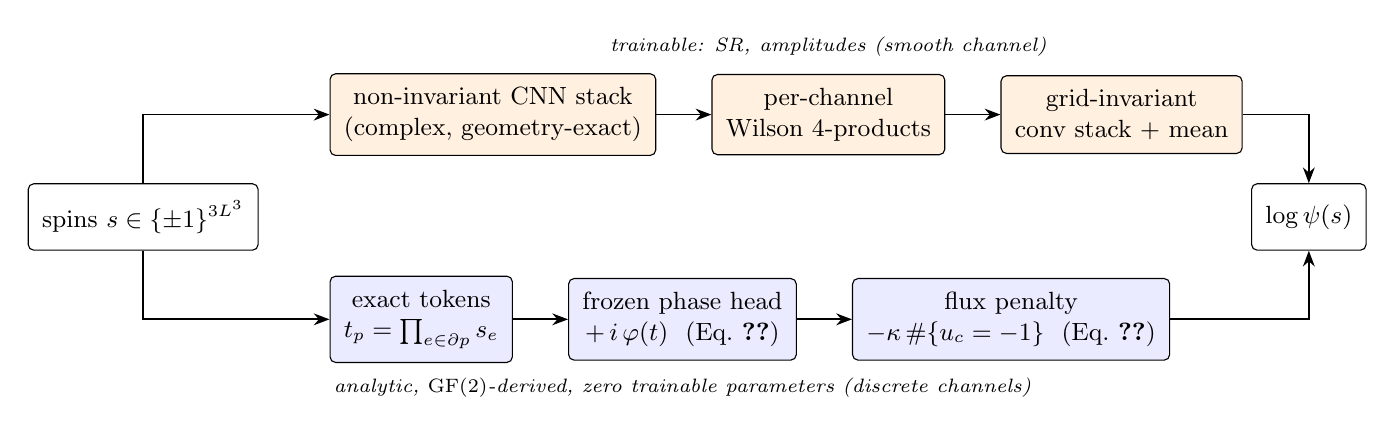
\begin{tikzpicture}[
  box/.style={draw, rounded corners=2pt, align=center, font=\small,
              inner sep=5pt, minimum height=2.4em},
  frozen/.style={box, fill=blue!8},
  train/.style={box, fill=orange!12},
  lbl/.style={font=\scriptsize\itshape},
  arr/.style={-{Stealth[length=2mm]}, semithick},
  node distance=5mm and 7mm]
\node[box] (in) {spins $s\in\{\pm1\}^{3L^3}$};
\node[train, right=9mm of in, yshift=13mm] (trunk)
  {non-invariant CNN stack\\(complex, geometry-exact)};
\node[train, right=of trunk] (wil) {per-channel\\Wilson $4$-products};
\node[train, right=of wil] (inv) {grid-invariant\\conv stack + mean};
\node[frozen, right=9mm of in, yshift=-13mm] (tok)
  {exact tokens\\$t_p=\prod_{e\in\partial p}s_e$};
\node[frozen, right=of tok] (head)
  {frozen phase head\\$+\,i\,\varphi(t)$ \ (Eq.~\ref{eq:head})};
\node[frozen, right=of head] (pen)
  {flux penalty\\$-\kappa\,\#\{u_c=-1\}$ \ (Eq.~\ref{eq:penalty})};
\node[box] (sum) at ($(inv.east)!0.5!(pen.east)+(13mm,0)$)
  {$\log\psi(s)$};
\draw[arr] (in) |- (trunk);
\draw[arr] (trunk) -- (wil);
\draw[arr] (wil) -- (inv);
\draw[arr] (in) |- (tok);
\draw[arr] (tok) -- (head);
\draw[arr] (head) -- (pen);
\draw[arr] (inv) -| (sum);
\draw[arr] (pen) -| (sum);
\node[lbl, above=1mm of wil] {trainable: SR, amplitudes (smooth channel)};
\node[lbl, below=1mm of head] {analytic, $\GF$-derived, zero trainable
parameters (discrete channels)};
\end{tikzpicture}%
}
\caption{The production fermionic ansatz: \texttt{ToricCNN\_gridinv} in
\file{tc3d/networks.py}, with \texttt{--phase\_head\_frozen} and
\texttt{--flux\_penalty}. The trunk is the standard complex gridinv CNN;
the token branch reads the \emph{raw} spins, so its two heads are exactly
the quadratic form \eqref{eq:quadform} and the sector projection
\eqref{eq:penalty}, independent of anything training does.}
\label{fig:stack}
\end{figure}

\subsection{Operational lessons worth keeping}
\label{sec:lessons}

Three production findings from 08-07..10 that are conceptual, not just
bug fixes.

\paragraph{(i) Checkpoints carry configuration, not just weights.}
The first $L=3$ gradient OOMed at 78\,GB, identically, three times, while
every plausible cause was eliminated in turn (the phase-head einsum ---
rewritten to the $(t\,Q)\odot t$ form anyway, commit \texttt{e3dba3c} --- was a
red herring). The real cause: NetKet's MCState serialization includes the
sampling configuration (\texttt{n\_samples}, \texttt{chunk\_size}, \dots), and
a raw \texttt{from\_bytes} warm start silently \emph{restored the
checkpoint's} --- so every \texttt{--init\_from} run inherited
\texttt{chunk\_size=None} from CPU-built pre-fit checkpoints and compiled the
unchunked kernel. Diagnostic fingerprint for the future: the allocation size
does not respond to the chunk setting, and the XLA log shows
\texttt{jit(forces\_expect\_hermitian)} without the \texttt{\_chunked}
suffix. Fixed in \file{tc3d/io.py} (\texttt{load\_weights} preserves the
caller's sampling config; commit \texttt{4d3d479}). Related sizing rule: the
fermionic Hamiltonian has $n_{\mathrm{conn}}\approx4L^3$ connected elements
per configuration, so chunking matters much earlier than in the bosonic
model (CHUNK 256 at $L=3$, $\sim$64--128 at $L=4$) --- and an unchunked $L=2$
success proves nothing about $L\ge3$.

\paragraph{(ii) Evaluate all Gauss laws as one matmul.}
The penalty masks are \emph{dense} ($\sim N_p/2$ tokens each), and the first
implementation evaluated one product kernel per mask: at $L=6$ (290 masks of
$\sim$324 tokens) this costs 78 \emph{minutes} per step. The production form
(commit \texttt{8986de0}) computes all parities in one fused matmul,
$\sum_c u_c = \sum_c\cos(\pi\,(b\,W)_c)$ with $b$ the token bits --- the sums
are exact integers in float64, so the $\pm1$ is exact to $\sim10^{-13}$.
Bit-identical on the $L=3$ probe ($-107.916(31)$, on-orbit weight 1.0000).

\paragraph{(iii) Chains must \emph{start} in the physical sector.}
The penalty makes ghost sectors improbable but does not teleport chains out
of them: a chain in a ghost coset must descend its violation count by local
moves, and that count has single-flip local minima. At $L=4$ a fraction of
randomly initialized chains stayed stuck and the energy error froze at
$7.3\times10^{-3}$ for 120 steps with constant sample spread.
\texttt{--chains\_up} initializes every chain at the all-up state --- zero
violations by construction --- \emph{after} \texttt{--init\_from}/resume, so a
restored sampler state cannot reintroduce stuck chains. ($L=2$ smoke:
$\delta=2.6\times10^{-4}$ at step 0.) The general lesson: an energy penalty
shapes the stationary distribution, not the ergodicity; sector membership
must be handled at initialization too.

\subsection{Status: the $L=4/5/6$ ladder}
\label{sec:status}

With frozen analytic heads (certified at these sizes), one-matmul penalties,
and \texttt{--chains\_up}, amplitude-only SR runs are in flight against the
exact anchors $E_0=-4L^3$:

\begin{center}
\begin{tabular}{@{}lccc@{}}
\toprule
& $L=4$ & $L=5$ & $L=6$\\
\midrule
exact $E_0$ & $-256$ & $-500$ & $-864$\\
final $E$ & [PENDING] & [PENDING] & [PENDING]\\
$\delta$, Vscore & [PENDING] & [PENDING] & [PENDING]\\
\bottomrule
\end{tabular}
\end{center}

\noindent
Nothing in the construction is size-specific anymore --- the only open
questions at large $L$ are optimization-and-throughput ones (chunking,
walltime, sampler mixing), which is exactly where the bosonic experience
transfers.

%=====================================================================
\section{The perturbed fermionic TC: design discussion for plan item
\texorpdfstring{\circled{3}}{(3)}}
\label{sec:finitefield}

This is the forward-looking part, framed as the design discussion for plan
item \circled{3}, the finite-field program
(\file{notes/fermionic\_next\_steps.md}), where QMC is sign-blocked and NQS
is the only method in town. The organizing
question: \emph{which parts of the $h=0$ solution are exact structure, which
become inductive bias, and which become wrong?}

\subsection{What survives at $h\neq0$: exactness degrades to initialization}
At any finite field the ground state is no longer a stabilizer state: the
quadratic-form sign structure and the flux-sector purity are the $h\to0$
limits, not identities. The frozen head and penalty therefore change status
--- from exact structure to \emph{exact initialization and inductive bias}.
This is the good scenario, and there is precedent: the bosonic $h_y\neq0$
runs \cite{SignNote} showed that a sign-full target continuously connected to
the initialization trains without incident. The analytic head places the
$h\neq0$ start \emph{inside the basin} of the true state, which is precisely
what the cold fermionic start lacked.

\subsection{Where do perturbative sign corrections live?}
The smooth phase deformations at small $h$ belong in the \emph{trunk}, which
has complex weights and currently contributes zero phase at the $h=0$
optimum. This is the doctrine-compatible split: the discrete part of the
sign structure stays frozen in the head; the smooth deformation on top is
trainable trunk phase. The alternative --- unfreezing $\theta$ --- should be
resisted on three counts: it reintroduces an optimizer into the discrete
channel (inviting exactly the smearing and drift of
Sec.~\ref{sec:options}(a)); it adds $N_p^2$ parameters to the QGT
(Sec.~\ref{sec:frozen}); and it is redundant, since any smooth token-quadratic
phase correction is representable by the trunk anyway (the trunk sees the
tokens' generating features). If a genuinely token-quadratic \emph{smooth}
correction turns out to dominate, the disciplined middle ground would be a
separate small \emph{trainable} head added to the frozen one --- zero-init,
low-rank --- so the discrete data remains untouchable. Whether that is ever
needed is an empirical question for the first $L=2$ ED-benchmarked sweeps.

\paragraph{An observation worth pinning down first (new, to be verified).}
The two field terms are not symmetric with respect to our discrete
structures. The Gauss parities $u_c$ \eqref{eq:gausslaw} are products of
$\sz$; they commute with $\Av$, with every $\Bt$ (by construction of the null
space), and with the $h_z\sz$ term --- but not with $h_x\sx$ on the odd-covered
edges. So along the \emph{electric line} ($h_x=0$, $h_z$ swept) the flux
sectors remain exactly superselected at any $h_z$, and the penalty remains an
exact sector projection, not an approximation. Stronger: conjugating $H$ by
the diagonal unitary $U=\mathrm{diag}\,(-1)^{q(t(s))}$ --- i.e.\ the frozen
head itself --- turns every $\Bt$ matrix element within the physical sector
positive (the head was built so that $(-1)^{q(t\oplus Me_p)+q(t)}
=\varepsilon_p(s)$ there), while $\Av$ and the diagonal $h_z$ term are
unaffected. If this argument survives scrutiny, then \emph{on the whole
electric line the model is stoquastic in the head-rotated frame restricted to
the physical sector}: the frozen head's signs are exact at every $h_z$, not
just at $h_z=0$, and training there is genuinely amplitude-only. This claim
is cheap to test ($L=2$ fermionic ED along $h_z$, comparing exact phases to
the head) and, if true, makes the electric cut the natural first campaign:
the doctrine would hold \emph{exactly}, and any observed sign drift in
training would be a red flag rather than physics. The magnetic response
($h_x\neq0$) is where both discrete structures genuinely soften.

\subsection{The flux penalty at $h\neq0$}
Under $h_x\neq0$ the field mixes flux sectors (a single $\sx$ flips the four
tokens of the plaquettes containing that edge, generically off
$\mathrm{col}\,M$), so the physical ground state acquires perturbatively
small ghost-sector weight. A fixed $\kappa=6$ then clamps that weight at
$e^{-2\kappa}\approx6\times10^{-6}$ per violation --- fine deep in the
topological phase, a bias once true sector weight exceeds it. Options, in
increasing order of ambition:
\begin{enumerate}
\item \textbf{Fixed $\kappa$, accept the bias} --- correct to the order we can
resolve at small $h_x$; simplest; the $L=2$ ED reference quantifies the bias
directly.
\item \textbf{$\kappa$ as a single trainable scalar} --- one parameter, low
risk. Note this does \emph{not} violate the doctrine: at $h\neq0$ the
sector weight is a genuinely smooth quantity, so its knob belongs to the
smooth channel. The discrete content (the \emph{masks}) stays analytic.
\item \textbf{A $\kappa(h)$ schedule} along \texttt{--init\_from} field
chains (the hysteresis infrastructure exists), annealing from 6 toward 0 as
fields grow; drop the penalty entirely once fields dominate and the sector
structure is washed out.
\end{enumerate}
Whatever the choice, the penalty (with \texttt{--chains\_up}) retains an
\emph{ergodicity} role near $h=0$ regardless of physics: at small $h_x$ the
sector-changing moves are rare, and without the penalty the sampler
recreates the ghost-census pathology in softened form. Keep it on for
conditioning even where it is not strictly needed for correctness.

\subsection{Validation without QMC}
QMC is sign-blocked here --- that is the point of the program --- so the
validation ladder is:
\begin{itemize}
\item \textbf{$L=2$ fermionic ED references at finite field}
(\file{tests/colab\_exact\_diag.py} has the fermionic toggle; cluster/Colab
job, $2^{24}$ states). These anchor the small-$h$ regime and directly
calibrate the $\kappa$ bias and any trunk-phase drift.
\item \textbf{Low-field perturbative series} \`a la
\file{analysis/exact\_benchmarks.py}, extended to the fTC --- the same
``accuracy certificate'' methodology as the bosonic campaigns.
\item \textbf{Internal certificates}: Vscore, the variational upper-bound
property against known anchors, and $\mathrm{Im}\langle E\rangle\approx0$ ---
remembering the $L=3$ lesson that these are necessary, never sufficient
(Sec.~\ref{sec:ghost}); the sector census should join them as a standard
fermionic diagnostic.
\end{itemize}

\subsection{Observables: already instrumented}
The order-parameter machinery is ported (plan item \circled{4}, commit
\texttt{f7c48bc}): the \emph{dressed} Wilson loop and open fermion string
live in \file{tc3d/fm.py}, built on \texttt{dressed\_string} from
\file{tc3d/fermionic\_decoration.py} --- the bare
$\sz$ loop is not conserved in the fTC; the $\GF$-solved $\sx$ dressing
restores a conserved $\tilde W$, while the open string's obstruction leaves
exactly one flux per endpoint (localized as a 3-plaquette body-diagonal
cluster per endpoint, size-independent; weight-2 proven impossible) --- the
operational fingerprint of the fermion. The Fredenhagen--Marcu ratio built
from these is the fermionic $O_{\mathrm{FM}}$, dropping into the existing
extraction pipeline.

\subsection{The physics goal}
The question the program exists to answer: \emph{how does a genuine emergent
fermion condense, compared to the bosonic $e$-charge?} The bosonic benchmark
is sharp --- $h_z^c\approx0.194$ for $e$-condensation
\cite{Linsel2026,SignNote} --- and the fTC differs at $h=0$ by exactly one
universal fact (the point charge is a fermion; gap 8 vs.\ 4). A single
fermion cannot condense the way a boson does; the candidate scenarios ---
shifted transition, different order, pair condensation, or confinement
without condensation --- have distinct signatures in $O_{\mathrm{FM}}$,
$\langle\tilde W\rangle$, the energy derivative (transition-order
diagnostic), and field-path hysteresis, all of which the pipeline already
measures for the bosonic model.

%=====================================================================
\section{Questions for discussion}
\label{sec:questions}

For the \circled{3} kickoff, the decisions that actually need taste rather than
computation:

\begin{enumerate}
\item \textbf{Field path.} Start with the electric line ($h_x=0$, sweep
$h_z$), where the sector structure --- and, if the stoquasticity observation
of Sec.~\ref{sec:finitefield} holds, the entire sign structure --- stays
exact? Or go straight for the magnetic response where the new physics (and
the new failure modes) live?
\item \textbf{Verify the electric-line claim.} Is the head-rotated
stoquasticity argument airtight (in particular: does the ground state remain
in the $u\equiv+1$ sector at all $h_z$)? An $L=2$ ED check is cheap and
would upgrade the claim from ``observation'' to ``design theorem.''
\item \textbf{$\kappa$ policy.} Fixed 6 / trainable scalar / scheduled? What
ghost-weight tolerance do we accept before the $L=2$ ED says the bias
matters?
\item \textbf{Trunk-phase budget.} Do we let the trunk carry all smooth
phase corrections (default), and what drift diagnostic distinguishes
``trunk learning legitimate $O(h)$ phases'' from ``trunk eroding the frozen
structure''? (Candidate: track head-vs-total phase decomposition on a fixed
probe set, plus the sector census.)
\item \textbf{Divergence guard.} The spike heuristic vetoes legitimate phase
restructuring in fermionic runs (established at $h=0$); what should the
production guard settings be for field sweeps, where some restructuring is
physical?
\item \textbf{Validation order.} Do we gate the first sweeps on the $L=2$
fermionic ED references (cluster job), or launch $L=2$ NQS sweeps and ED in
parallel and reconcile after?
\item \textbf{Even-$L$ compression (optional).} Is the seam-decorated
stencil (TI stencil + Kasteleyn-style defect plane,
Sec.~\ref{sec:stencil}) worth pursuing for memory at $L\ge8$, or does the
dense frozen head (free at runtime, $O(N_p^2)$ memory only) carry us through
the FSS window?
\end{enumerate}

%=====================================================================
\begin{thebibliography}{9}\small

\bibitem{SignNote}
\emph{The sign problem of the 3D fermionic toric code: background, mechanism,
and consequences for NQS}, project note
\file{notes/fermionic\_sign\_problem.tex} (2026-08-07). Background and
notation for the present document; see also
\file{notes/fermionic\_plateau\_diagnosis.md} and
\file{notes/handoff\_fermionic\_tc.md}.

\bibitem{SzaboCastelnovo2020}
A.~Szab\'o and C.~Castelnovo,
\emph{Neural network wave functions and the sign problem},
Phys.\ Rev.\ Research \textbf{2}, 033075 (2020), arXiv:2002.04613.

\bibitem{ChenKapustinRadicevic2018}
Y.-A.~Chen, A.~Kapustin, and D.~Radi\v{c}evi\'c,
\emph{Exact bosonization in two spatial dimensions and a new class of lattice
gauge theories}, Ann.\ Phys.\ \textbf{393}, 234 (2018), arXiv:1711.00515.

\bibitem{ChenKapustin2019}
Y.-A.~Chen and A.~Kapustin,
\emph{Bosonization in three spatial dimensions and a 2-form gauge theory},
Phys.\ Rev.\ B \textbf{100}, 245127 (2019), arXiv:1807.07081.

\bibitem{LevinWen2003}
M.~Levin and X.-G.~Wen,
\emph{Fermions, strings, and gauge fields in lattice spin models},
Phys.\ Rev.\ B \textbf{67}, 245316 (2003).

\bibitem{Linsel2026}
S.~M.~Linsel, L.~Pollet, and F.~Grusdt,
\emph{(QMC phase diagram of the 3D toric code in a field; project benchmark
reference)}, PRX Quantum \textbf{7}, 010332 (2026).

\end{thebibliography}

\end{document}
